\documentclass[11pt,aspectratio=169]{beamer}

%%==============================================================================
%% Header
%%==============================================================================

\usetheme{metropolis}
\setsansfont{Source Sans Pro}
\setmonofont{Source Code Pro}

\hypersetup{colorlinks=true,
            linkcolor=mRustLightOrange,
            menucolor=mRustLightOrange,
            pagecolor=mRustLightOrange,
            urlcolor=mRustLightOrange}
\usepackage{csquotes}
\usepackage{comment}
\usepackage{xcolor}
\usepackage{minted}
\usepackage{pdfpages}
\usepackage{pdfcomment}
\usepackage{mathtools}
\usepackage{listings}

\definecolor{mRustDarkOrange}{HTML}{8d2f00}
\definecolor{mRustLightOrange}{HTML}{ff9600}
\definecolor{errMsg}{HTML}{CC1100}
\definecolor{warnMsg}{HTML}{EE9900}
\definecolor{refMsg}{HTML}{0011CC}
\definecolor{linkColor}{HTML}{006600}
\definecolor{urlColor}{HTML}{006600}
\hypersetup{colorlinks=true,linkcolor=linkColor,urlcolor=urlColor}

\let\orignote\note
\renewcommand<>{\note}[1]{\only#2{\tikz[remember,picture,overlay]{\node{\pdfmargincomment[opacity=0]{#1}}}}\orignote#2{#1}}

\AtBeginEnvironment{minted}{%
  \renewcommand{\fcolorbox}[4][]{#4}}

\newfontfamily\codefont{Source Code Pro}
\newcommand\code[1]{\,{\color[HTML]{884400}#1}\,}
\newcommand\source[1]{$\rightarrow$ via #1}

\title{Rust and memory safety}
\subtitle{\small{\url{https://lukas-prokop.at/talks/2021-11-30_rustgraz}}}
\date{\today}
\author{Lukas Prokop}
\institute{RustGraz community 
\includegraphics[height=.5cm]{../images/rustacean-orig-noshadow.png}}

\begin{document}
\maketitle

%==============================================================================
% Title
%==============================================================================

\begin{frame}[fragile]{rust overview}
  \begin{enumerate}
    \item \hyperlink{intro}{Introduction to rust}
      \begin{itemize}
        \item
          \hyperlink{type-suffixes}{type suffixes},
          \hyperlink{func}{functions},
          \hyperlink{anon}{anonymous functions},
          \hyperlink{trait}{traits},
          \hyperlink{mod}{modularization},
          \hyperlink{arrays}{arrays and slices}
      \end{itemize}
    \item Software development practices
      \begin{itemize}
        \item
          \hyperlink{pattern-matching}{Pattern matching and error handling}, 
          \hyperlink{macros}{macros}, 
          \hyperlink{typestate}{typestate pattern}, 
          \hyperlink{ref}{references}
          %Advanced types
      \end{itemize}
    \item memory safety
      \begin{itemize}
        \item
          \hyperlink{xor}{Mutation xor aliasing},
          \hyperlink{ownership}{ownership model and borrowing}, 
          \hyperlink{unsafe}{unsafe superpowers}, 
          \hyperlink{ub}{undefined behavior}
      \end{itemize}
    \item \hyperlink{resources}{Resources}
  \end{enumerate}
\end{frame}

\label{intro}
\section{Introduction to rust}

\begin{frame}[fragile]{rust overview}
  \begin{columns}
    \begin{column}{0.7\textwidth}
      \begin{itemize}
        \item multi-paradigmatic \\ (imperative, functional)
        \item systems programming language \\ (easy interop with C, no GC)
        \item focus on memory safety and concurrency
        \item uses the LLVM infrastructure
        \item syntax similar to C++, immutability by default
        \item Modern competitors: Nim, Crystal, D, Zig, Go?
        \item 1.0 (May 2015), 1.56 (Rust 2021 edition, current)
      \end{itemize}
      \emph{\enquote{Most loved programming language}} \\
      (Stack Overflow Developer Survey, 2016--2021)
    \end{column}
    \begin{column}{0.3\textwidth}
      \begin{center}
        
\includegraphics[width=\textwidth]{../images/rust_logo_wikipedia.pdf}
      \end{center}
    \end{column}
  \end{columns}
\end{frame}

% Q Which functional programming languages did you use in your life so far?

\label{type-suffixes}
\begin{frame}[fragile]{rust type suffixes}
  \newcommand\showtype[1]{\textbf{\texttt{\color{mRustLightOrange}#1}}\hspace{15pt}}
  \begin{center}
    \showtype{u8} \showtype{u16} \showtype{u32} \showtype{u64} \showtype{u128} \\
    \showtype{i8} \showtype{i16} \showtype{i32} \showtype{i64} \showtype{i128} \\
    \showtype{isize} \showtype{usize} \showtype{f32} \showtype{f64} \\
    \showtype{bool} \showtype{char}
  \end{center}
  → type suffix notation: \mintinline{rust}{42u8}
  \begin{minted}{rust}
42   42_000   0xFF   0o777   0b0010_1010  std::u32::MAX
1.   1e6   -4e-4f64  std::f64::INFINITY   std::f64::NAN
1usize   true   false  'c'
  \end{minted}
  → type inference to determine data type \\
  → default integer type is i32
\end{frame}

\label{func}
\begin{frame}[fragile]{rust functions}
  \begin{minted}[linenos=true]{rust}
fn square(arg: f64) -> f64 {
  arg * arg
}

fn main() {
  let a: f64 = 2.1;
  println!("the square of {} is {}", a, square(a));
}
  \end{minted}
\end{frame}

\label{anon}
\section{Anonymous functions}

\begin{frame}[fragile]{Function syntax}
  \begin{minted}{rust}
fn named(name1: T1, name2: T2) -> T_RETURN {}
let unnamed = |name1: T1, name2: T2| -> T_RETURN { };
let short   = |name1    , name2    |             { };
  \end{minted}
\end{frame}

\begin{frame}[fragile]{Function syntax}
  Example of anonymous function usage:
  \begin{minted}{rust}
use std::thread;
let handler = thread::spawn(|| {
    println!("Hello World!");
});
handler.join().unwrap();
  \end{minted}
\end{frame}

\label{trait}
\begin{frame}[fragile]{traits}
  \begin{minted}[fontsize=\small]{rust}
trait Submission {
  fn len(&self) -> u32;
  fn summary(&self) -> String;
}
  \end{minted}
  \begin{itemize}
    \item \texttt{trait}s are inspired by Haskell typeclasses (no subtyping); like interfaces
    \item Nominal type system (like C++/Java/C\#), not structural type system (like Go)
    \item default implementations and constant attributes can be provided
    \item \texttt{struct}s, \texttt{enum}s, and \texttt{union}s can implement traits
    \item first parameter is not \mintinline{rust}{&self}? Then static method
    \item Implementing \mintinline{rust}{std::ops::Add}? Enables \texttt{+} (operator overloading)
  \end{itemize}
\end{frame}

\begin{frame}[fragile]{trait implementation}
  \begin{minted}[linenos=true,fontsize=\scriptsize]{rust}
struct Talk {
  desc: String,
  duration: u16,
}
impl Submission for Talk {
  fn len(&self) -> u32 { self.duration as u32 }
  fn summary(&self) -> String {
    let dot = self.desc.find('.');
    match dot {
      Some(idx) => {
        let mut s = String::new();
        s.push_str(&self.desc[0..idx]);
        s.push_str(" …");
        s
      },
      None => self.desc.clone(),
} } }
  \end{minted}
\end{frame}

\label{mod}
\begin{frame}[fragile]{modularization}
  \begin{minted}[linenos=true,fontsize=\small]{rust}
use std::vec::Vec as V;
pub fn exclaim(x: &&str) -> String {
  let mut s = x.to_string();
  s.push_str("!");
  s
}
pub fn hash_map_example() {
  let calls: V<&str> = vec!["Hey", "You"];
  let shouts = calls.iter().map(exclaim);
  println!("He shouted: {}", shouts.collect::<V<String>>().join(" "));
}
  \end{minted}
  \vspace{-3pt}
  \begin{enumerate}
    \item \mintinline{rust}{use} for import, \mintinline{rust}{as} for renaming
    \item functional elements like map, zip, filter
    \item \mintinline{rust}{pub} to expose functions publicly, modules are called \href{https://crates.io/}{crates}
  \end{enumerate}
\end{frame}

\label{arrays}
\section{Arrays}

\begin{frame}[fragile]{Arrays}
  \begin{minted}[linenos=true]{rust}
// declaration and initialization
let mut array: [u32; 3] = [0; 3]; // [{init-value}; {length}]

// iterate over an array
for x in array.iter() { }

// indexing and assignment
array[1] = 1;
array[2] = 2;
\end{minted}
\end{frame}

\begin{frame}[fragile]{Arrays}
  \begin{itemize}
    \item Arrays (like \mintinline{rust}{[u8; 42]}) have a known, fixed size
    \item Arrays need to be initialized
          \begin{itemize}
            \item compile time checks
            \item exceptions via \href{https://doc.rust-lang.org/std/mem/union.MaybeUninit.html}{MaybeUninit}
          \end{itemize}
    \item Memory layout: consecutive memory segment
    \item Few API limitations for arrays of length $>$32
  \end{itemize}
\end{frame}

% use std::default::Default;
% 
% fn main() {
%   let mut array1: [u32; 99] = Default::default();
%   let mut array2: [u32; 99] = [0; 99];
%   assert_eq!(array1, array2);
% }

\begin{frame}[fragile]{Slices}
  \begin{minted}{rust}
array[0..21]
\end{minted}
  \begin{itemize}
    \item Slices (like \mintinline{rust}{[u8]}) are memory views into an array
    \item Unknown size
    \item Memory layout: only a pointer
    \item Barely useful because they cannot be passed as fn argument or return value
  \end{itemize}
\end{frame}

\begin{frame}[fragile]{References to slices}
  \begin{minted}[linenos=true]{rust}
&array[0..21]
\end{minted}
  \begin{itemize}
    \item References to slices are references to memory views into an array
    \item \textbf{known} size, see \mintinline{rust}{len()} method
    \item Memory layout: pointer with length
    \item Similar performance characteristics like an array
  \end{itemize}
\end{frame}

\section{Software development practices}

\label{pattern-matching}
\section{Pattern matching and error handling}

\begin{frame}[fragile]{pattern matching}
  \begin{minted}[linenos=true]{rust}
fn main() {
  let course = "ssd";
  println!("{} ({})",
    match course {
      "ssd" => "Secure Software Development",
      _ => "unknown"
    },
    course.to_uppercase()
  );
}
  \end{minted}
\end{frame}

\begin{frame}[fragile]{algebraic data types}
  \begin{quote}
    In computer programming, especially functional programming and type theory,
    an \textbf{algebraic data type} (ADT) is a kind of composite type, i.e., a type formed by combining other types. \\
    ---\href{https://en.wikipedia.org/wiki/Algebraic_data_type}{Wikipedia}
  \end{quote}
\end{frame}

\begin{frame}[fragile]{Haskell's data and rust's enum}
  \begin{minted}{haskell}
data List a = Nil | Cons a (List a)
  \end{minted}
  \vspace{20pt}
  \pause
  \begin{minted}{rust}
enum List {
  Nil,
  Cons(Box<List>, u32),
}
\end{minted}
\end{frame}

\begin{frame}[fragile]{Haskell's data and rust's enum}
  \begin{minted}{haskell}
data Tree = Empty
          | Leaf Int
          | Node Tree Tree
  \end{minted}
  \vspace{20pt}
  \pause
  \begin{minted}{rust}
enum Tree {
  Empty,
  Leaf(u32),
  Node(Box<Tree>, Box<Tree>),
}
  \end{minted}
\end{frame}

\begin{frame}[fragile]{enum introduces an algebraic data type}
  \begin{itemize}
    \item Algebraic? Sums and products.
          \begin{itemize}
            \item \texttt{List} is the sum of \texttt{Nil} and \texttt{Cons(\_)}.
            \item \texttt{Cons} is the product of \texttt{Box$<$List$>$} and \texttt{u32}.
          \end{itemize}
    \item Boxing? Avoids \mintinline{text}{recursive type `List` has infinite size}.
    \item Article: \href{https://blog.softwaremill.com/algebraic-data-types-in-four-languages-858788043d4e}{Algebraic data types in four languages} (namely Haskell, Scala, rust, and TypeScript)
  \end{itemize}
\end{frame}

\begin{frame}[fragile]{pattern matching on enums}
  \begin{minted}[linenos=true]{rust}
impl fmt::Display for List {
  fn fmt(&self, f: &mut fmt::Formatter<'_>) -> fmt::Result {
    match self {
      List::Cons(inner, item)
        => write!(f, "(cons {} {})", item, inner),
      List::Nil
        => write!(f, "nil"),
    }
  }
}
  \end{minted}
  Recognize that \texttt{Cons} is addressed by \mintinline{rust}{List::Cons}.
\end{frame}

\begin{frame}[fragile]{Contrived error handling}
  \begin{minted}[fontsize=\scriptsize]{rust}
enum Result {
  Okay(Digest),
  Error(String),
}
\end{minted}
  \pause
  \begin{minted}[fontsize=\scriptsize]{rust}
fn generate_digest() -> Result {
  Result::Okay([42u8; 32])
}
\end{minted}
  \pause
  \begin{minted}[fontsize=\scriptsize]{rust}
fn main() {
  match generate_digest() {
    Result::Okay(d) => {
      for byte in d.iter() { print!("{:02X}", byte); }
      println!("");
    },
    Result::Error(msg) => eprintln!("error: {}", msg),
  }
}
  \end{minted}
\end{frame}

\begin{frame}[fragile]{Error handling in rust}
  \mintinline{rust}{std::result::Result<T, E>}
  \begin{itemize}
    \item \mintinline{rust}{Ok(T)}
    \item \mintinline{rust}{Err(E)}
  \end{itemize}
  No exceptions, no error codes.

  \vspace{20pt}
  \pause
  \mintinline{rust}{std::option::Option<T>}
  \begin{itemize}
    \item \mintinline{rust}{None}
    \item \mintinline{rust}{Some(T)}
  \end{itemize}
  If we fetch one element from a container data structure, \\
  we get \emph{some} value or \emph{none}.
\end{frame}

\begin{frame}[fragile]{Error handling in rust}
  \begin{minted}{rust}
// Example for Result
match File::open("foo.txt") {
  Ok(fd) => { /* ... */ },
  Err(e) => panic!(e),
}

// Example for Some
let fetched = Some(value);
fetched.unwrap();  // return Some value or panic
fetched.unwrap_or(default_value);  // … or default
\end{minted}
  You usually implement error types (SyntaxError, InvalidArgError, \dots) on your own in your library.
\end{frame}

\begin{frame}[fragile]{Error handling in rust}
  \begin{minted}[fontsize=\small]{rust}
// Result API (excerpt)
fn is_ok(&self) -> bool;
fn is_err(&self) -> bool;
fn ok(self) -> Option<T>;
fn err(self) -> Option<E>;
fn and_then<U, F>(self, op: F) -> Result<U, E>;

// Option API (excerpt)
fn is_some(&self) -> bool;
fn is_none(&self) -> bool;
fn unwrap(self) -> T;
fn unwrap_or(self, default: T) -> T;
fn ok_or<E>(self, err: E) -> Result<T, E>;
\end{minted}
\end{frame}

\begin{frame}[standout]
  \begin{center}
    \vspace{1.5cm}
    {\Huge rust has a unique error handling operator}
  \end{center}
\end{frame}

\begin{frame}[fragile]{Question mark operator}
  The question mark operator exits early in case of \mintinline{rust}{Err}
  or returns the value otherwise.
  \begin{minted}[linenos=true]{rust}
fn compile(src: &str) -> Result<(), Error> {
  let tokens = tokenize(&src)?;
  let ast = parse(&tokens)?;
  // …
  Ok(())
}
  \end{minted}
  Return type of function must be a corresponding \mintinline{rust}{Result}.
\end{frame}

\begin{frame}[fragile]{Question mark operator rewritten}
  It is can be rewritten with a match expression:
  \begin{minted}[linenos=true]{rust}
fn compile(src: &str) -> Result<(), Error> {
  let tokens = match tokenize(&src) {
    Err(E) => return Err(E),
    Ok(ts) => ts,
  };
  let ast = parse(&tokens)?;
  // …
  Ok(())
}
  \end{minted}
\end{frame}

\label{macros}
\section{Macros}

\begin{frame}[fragile]{Macros}
  \begin{itemize}
    \item Three kinds of macros
          \begin{enumerate}
            \item function-like macros (\mintinline{rust}{println!("hi")})
            \item derive macros (\mintinline{rust}{derive(Debug)})
            \item attribute-like macros (\mintinline{rust}{cfg(target_arch = "x86")})
          \end{enumerate}
  \end{itemize}

  \textbf{Important differences from C:}
  \begin{itemize}
    \item They operate on tokens, not the lexical level
    \item Macro hygiene (variables are not visible outside)
  \end{itemize}
\end{frame}

\begin{frame}[fragile]{Macros}
  \begin{minted}[escapeinside=~~,fontsize=\small]{rust}
~\textbf{macro\_rules}~! shake {
  (update $base:ident with $($elem:expr, )*)
    => { $( $base.update($elem); )* };
}
  \end{minted}
  \begin{minted}[escapeinside=~~,fontsize=\small]{text}
~\textbf{Input:}~
  shake!(update h with &data, &[b' '], &data2,);
  \end{minted}
  \begin{minted}[escapeinside=~~,fontsize=\small]{text}
~\textbf{Output:}~
  h.update(&data);
  h.update(&[b' ']);
  h.update(&data2);
  \end{minted}
  %\talknote{macros can access and adjust AST}
  %\talknote{tokens, not lexical level; whitespace is more limited}
  %\talknote{macro hygiene}
\end{frame}

\label{typestate}
\section{typestate pattern}

\begin{frame}[fragile]{The typestate pattern}
  \textbf{Idea:} Encode the state in the type

  \textbf{Example:}
  \begin{itemize}
    \item \texttt{fopen} returns \texttt{FileOpened}
    \item \texttt{fwrite} returns \texttt{FileNonEmpty}
    \item \texttt{fclose} returns \texttt{FileClosed}
  \end{itemize}

  More details, for example, in \href{http://cliffle.com/blog/rust-typestate/}{The Typestate Pattern in Rust} (blog post).
\end{frame}

\begin{frame}[fragile]{The typestate pattern}
  \textbf{Why?} Can increase security.
  \vspace{20pt}

  \begin{quote}
    Both from a design point of view as from an implementation perspective the entire scope can be considered of exceptionally high standard. Using the type system to \textbf{statically encode properties such as the TLS state transition function} is one just one example of great defense-in-depth design decisions. \\
    ---\href{https://github.com/ctz/rustls/blob/master/audit/TLS-01-report.pdf}{rustls formal audit report}
  \end{quote}
\end{frame}

\label{ref}
\section{References}

\begin{frame}[fragile]{Shared references in rust}
  \begin{minted}{rust}
fn main() {
  let mut a = 42u32;
  let b: &u32 = &a;
  
  println!("value of ref: {}", *b);
}
  \end{minted}
  \begin{itemize}
    \item \texttt{b} is a [shared] reference (\mintinline{rust}{&u32}) to \texttt{a}.
    \item Reference operator \texttt{\&}
    \item Dereference operator \texttt{*}
  \end{itemize}
\end{frame}

\begin{frame}[fragile]{Mutable references in rust}
  \begin{minted}{rust}
fn main() {
  let mut a = 42u32;
  let b: &mut u32 = &mut a;
  
  *b = 2;
  println!("value of ref: {}", *b);
}
  \end{minted}
  \begin{itemize}
    \item \texttt{b} is a [\emph{mutable}] reference (\mintinline{rust}{&u32}) to \texttt{a}.
    \item Reference operator \mintinline{rust}{&mut}
    \item Dereference operator \texttt{*}
  \end{itemize}
\end{frame}

\begin{frame}[fragile]{Auto-dereferencing in rust}
  \begin{minted}{rust}
fn main() {
  let mut a = 42u32;
  let b: &u32 = &a;
  
  println!("value of ref: {}", b);
}
  \end{minted}
  Recognize that \texttt{b} does not need the dereference operator.
  Rust implements \emph{auto-dereferencing}.
  Best practice: write derefs explicitly.
\end{frame}

% TODO advanced types










\label{memory-safety}
\section{Memory safety}


{
\setbeamercolor{background canvas}{bg=}
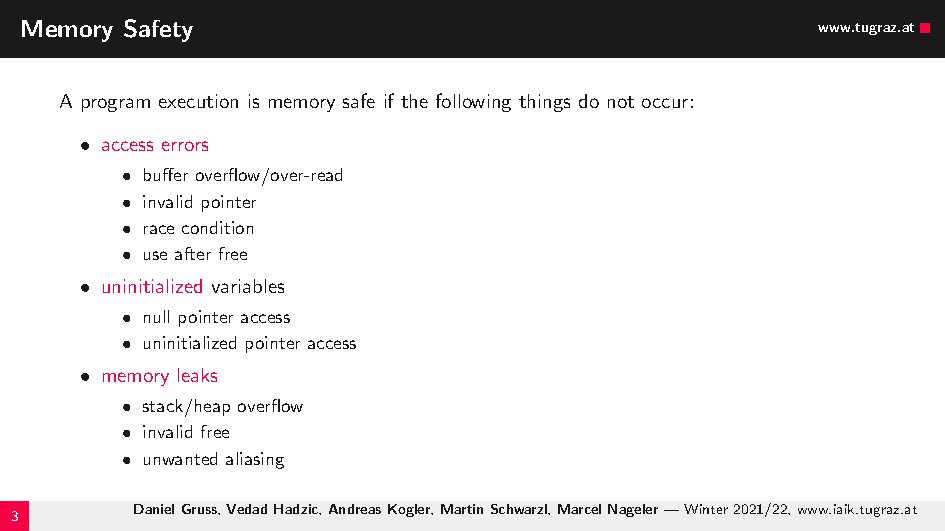
\includepdf{02-memory_corruption_1_examples}
}

\label{xor}
\section{Mutation xor aliasing}

\begin{frame}[fragile]{References}
  Rules:
  \begin{itemize}
    \item one or more \emph{shared} references (\mintinline{rust}{&T}) to a resource
    \item exactly one \emph{mutable} reference (\mintinline{rust}{&mut T})
    \item either or, not both! (\enquote{aliasing xor mutation})
  \end{itemize}

  Benefits of reference limitations for memory safety:
  \begin{itemize}
    \item one writer XOR n readers in concurrent context
    \item prevents data races
  \end{itemize}
\end{frame}

\label{ownership}
\section{Ownership and borrowing}

\begin{frame}[fragile]{Ownership}
  C++ uses the notion of \href{https://en.wikipedia.org/wiki/Resource_acquisition_is_initialization}{RAII}:
  \begin{minted}[fontsize=\small]{cpp}
void WriteToFile(const std::string& message) {
  static std::mutex mutex;
  std::lock_guard<std::mutex> lock(mutex);
  std::ofstream file("example.txt");
  if (!file.is_open()) {
    throw std::runtime_error("unable to open file");
  }
  file << message << std::endl;
}
  \end{minted}
\end{frame}

\begin{frame}[fragile]{Ownership}
  \begin{itemize}
    \item Each value in Rust has a variable that’s called its \emph{owner}
    \item There can only be one owner at a time
    \item Ownership can \emph{move} from one variable to another
    \item When the owner goes out of scope, the value will be \enquote{dropped}
  \end{itemize}
\end{frame}

\begin{frame}[fragile]{Ownership example}
  \begin{minted}[fontsize=\footnotesize]{rust}
#[derive(Debug)]
struct Stats { score: u32 }

fn sub(mut s: Stats) {
  s.score += 1;
}

fn main() {
  let a = Stats { score: 8 };
  sub(a);

}
  \end{minted}
  % Recognize that a is immutable, s is mutable
\end{frame}

\begin{frame}[fragile]{Ownership example}
  \begin{minted}[fontsize=\footnotesize]{rust}
#[derive(Debug)]
struct Stats { score: u32 }

fn sub(mut s: Stats) {
  s.score += 1;
}

fn main() {
  let a = Stats { score: 8 };
  sub(a);
  println!("{:?}", a);
}
  \end{minted}
\end{frame}

\begin{frame}[fragile]{Ownership example}
  \begin{minted}[escapeinside=~~,fontsize=\footnotesize]{text}
~\color{errMsg}{error[\textbf{E0382}]: borrow of moved value: `a`}~
  ~\color{refMsg}{--> src/main.rs:10:20}~
   |
8  |     ~\textbf{let a = Stats \{ score: 8 \};}~
   |         - move occurs because `a` has type `Stats`,
   |           which does not implement the `Copy` trait
9  |     ~\textbf{sub(a);}~
   |         - value moved here
10 |     ~\textbf{println!("\{\}", a);}~
   |                    ^
   |         value borrowed here after move
  \end{minted}
\end{frame}

\begin{frame}[fragile]{Ownership example}
  \begin{minted}[fontsize=\footnotesize]{rust}
#[derive(Debug)]
struct Stats { score: u32 }

fn sub(mut s: Stats) {
  // owner of Stats instance = `s`
  s.score += 1;
  // `s` goes out of scope → Stats instance is dropped
}

fn main() {
  let a = Stats { score: 8 };
  // owner of Stats instance = `a`
  sub(a); // move Stats instance: `a` → `s`
  println!("{:?}", a); // has been dropped already → error
}
  \end{minted}
\end{frame}

\begin{frame}[fragile]{Ownership example}
  Solutions:
  \begin{itemize}
    \item Use \mintinline{rust}{#[derive(Debug,Copy,Clone)]}. Then \mintinline{text}{sub} uses copied instance. Results in \mintinline{rust}{Stats { score: 8 }}
    \item Return \mintinline{text}{Stats} instance and assign it again in \mintinline{text}{main}.
    \item Use references (\emph{borrowing} ownership)
  \end{itemize}

  Benefits of ownership for memory safety:
  \begin{itemize}
    \item we can pin-point when a variable is dropped (across threads!)
  \end{itemize}
\end{frame}

\begin{frame}[fragile]{Ownership example with borrowing}
  \begin{minted}[fontsize=\footnotesize]{rust}
#[derive(Debug)]
struct Stats { score: u32 }

fn sub(s: &mut Stats) {
  s.score += 1;
}

fn main() {
  let mut a = Stats { score: 8 };
  // ownership of `a` is borrowed to `s`
  sub(&mut a);
  // ownership of `s` is returned back to `a`
  println!("{:?}", a);
}
  \end{minted}
\end{frame}

\label{unsafe}
\section{unsafe superpowers}

\begin{frame}[fragile]{unsafe}
  \begin{minted}[fontsize=\footnotesize]{rust}
#[cfg(any(target_arch = "x86", target_arch = "x86_64"))]
fn rdtscp() -> (u64, u32) {
  let (mut eax, mut ecx, mut edx) = (0, 0, 0);
  {
    unsafe {
      asm!(
        "rdtscp",
        lateout("eax") eax,
        lateout("ecx") ecx,
        lateout("edx") edx,
        options(nomem, nostack)
      );
    }
} }
  \end{minted}
  \href{https://lukas-prokop.at/articles/2021-11-10-rdtsc-with-rust-asm}{Blog article: Intel's RDTSC instruction with rust's RFC-2873 asm! macro}
\end{frame}

\begin{frame}[fragile]{unsafe}
  \textbf{Superpowers:}
  \begin{enumerate}
    \item Dereference a raw pointer (\mintinline{rust}{const *})
    \item Call an \mintinline{rust}{unsafe} function or method
    \item Access or modify a mutable static variable
    \item Implement an \mintinline{rust}{unsafe} trait
    \item Access fields of \mintinline{rust}{unions}
  \end{enumerate}
\end{frame}

\begin{frame}[fragile]{Abusing unsafe}
  \begin{minted}[linenos=true,fontsize=\footnotesize]{rust}
fn get_mutable_ref(val: &u32) -> &mut u32 {
  let ptr: *const u32 = val;
  let ptr_mut: *mut u32 = ptr as *mut u32;
  let ref_mut: &mut u32 = unsafe { &mut *ptr_mut };
  ref_mut
}
fn demo_two_mutable_refs() {
  let v: u32 = 42;
  let ref1: &mut u32 = get_mutable_ref(&v);
  let ref2: &mut u32 = get_mutable_ref(&v);

  *ref1 = 13;
  assert_eq!(*ref2, 13);
  *ref2 = 7;
  assert_eq!(*ref1, 7);
}
  \end{minted}
\end{frame}

\label{ub}
\section{Does UB exist in rust?}

\begin{frame}[fragile]{UB in rust}
  \begin{itemize}
    \item Not all bugs can be caught with the type system
    \item A type system needs to be relaxed to be pragmatic
    \item A type system needs to be strict to be able to reason about it
  \end{itemize}
  \textbf{Does undefined behavior (UB) exist in rust?} Yes.
  \begin{itemize}
    \item See \href{https://doc.rust-lang.org/beta/reference/behavior-considered-undefined.html}{Behavior considered undefined} for a non-exhaustive list
    \item Corner cases are still subject to academic debate
  \end{itemize}
\end{frame}

\begin{frame}[fragile]{Overflow snippet}
  The following snippet can trigger an overflow. Where?

  \begin{lstlisting}[language={C}]
char buffer[128];
int bytesToCopy = packet.length;
if (bytesToCopy < 128) {
    strncpy(buffer, packet.data, bytesToCopy);
}
  \end{lstlisting}
  Example via \href{https://reberhardt.com/cs110l/spring-2020/slides/lecture-01.pdf}{CS 110L, Ryan Eberhardt and Armin Namavari}
  \pause
  \begin{itemize}
    \item Proper bounds check (yay!)
    \item \texttt{strncpy}, not \texttt{strcpy} (yay!)
  \end{itemize}
\end{frame}

\begin{frame}[fragile]{Overflow snippet solved}
  The issue:
  \begin{enumerate}
    \item As declared, \mintinline{C}{bytesToCopy} is an \texttt{int}
    \item Third argument of \texttt{strncpy} is a \texttt{size\_t}
    \item \mintinline{C}{bytesToCopy < 128} is true if \texttt{bytesToCopy} is negative
    \item \mintinline{C}{bytesToCopy} is cast to an unsigned type and becomes huge
  \end{enumerate}
  How is this prevented in rust?
  \begin{itemize}
    \item Types contain length (\mintinline{rust}{String} is \mintinline{rust}{Vec<u8>}, a \mintinline{rust}{Vec} carries a \texttt{len})
    \item No implicit casts (explicit casts via \mintinline{rust}{as})
    \item Bounds checks: arrays are sized anyways, but other container per default use bound checks
  \end{itemize}
\end{frame}


\label{resources}
\section{Resources}

\begin{frame}[fragile]{Rust for beginners}
  I mostly used the \href{https://doc.rust-lang.org/stable/book/}{rust book}.
  \begin{itemize}
    \item \href{https://www.forrestthewoods.com/blog/learning-rust-via-advent-of-code/}{Learning Rust via Advent of Code}
    \item \href{https://github.com/rust-lang/rustlings}{Small exercises to get you used to reading and writing Rust code}
    \item \href{https://doc.rust-lang.org/rust-by-example/}{Rust by example}
    \item \href{https://www.rust-lang.org/learn}{Rust official doc}
    \item \href{https://doc.rust-lang.org/std/index.html}{stdlib}
    \item \href{https://github.com/mre/idiomatic-rust}{Idiomatic rust}
    \item \href{https://fasterthanli.me/blog/2020/a-half-hour-to-learn-rust/}{A half hour to learn rust}
  \end{itemize}
\end{frame}

\begin{frame}[fragile]{Tools}
  \begin{description}
    \item[\href{https://github.com/rust-lang/rust-clippy}{clippy}] detects common mistakes and unidiomatic code
    \item[\href{https://github.com/rust-lang/rustfmt}{rustfmt}] allows you to reformat/normalize rust source code
  \end{description}
  There are many UNIX utilities rewritten in rust (\href{https://github.com/BurntSushi/xsv}{xsv}, \href{https://github.com/BurntSushi/ripgrep}{ripgrep}, etc.)
\end{frame}

\begin{frame}[fragile]{Rust at university}
  University courses on Rust:
  \begin{itemize}
    \item \href{https://github.com/LukasKalbertodt/programmieren-in-rust}{Rust course by Lukas Kalbertodt}
    \item \href{https://www.youtube.com/channel/UCRA18QWPzB7FYVyg0WFKC6g/videos}{CS196 at Illinois}
    \item \href{https://reberhardt.com/cs110l/spring-2020/}{CS110L at Stanford}
  \end{itemize}

  Academia:
  \begin{itemize}
    \item \href{http://plv.mpi-sws.org/rustbelt/}{RustBelt}: academic project for formal verification of the Rust compiler
  \end{itemize}
\end{frame}

\begin{frame}[standout]
  \begin{center}
    \vspace{1.5cm}
    Thank you! Q/A?

    
\includegraphics[width=0.4\textwidth]{../images/rustacean-flat-happy.png}
  \end{center}
\end{frame}

% TODO illustrate type inference better

\end{document}
